\documentclass[smallheadings,12pt]{scrartcl}
\usepackage{marvosym}
\usepackage{color}
\usepackage{float}
\usepackage{geometry}
\usepackage{graphicx}
\usepackage{soul} % underlining text
\geometry{verbose,letterpaper,tmargin=0cm,bmargin=3cm,lmargin=2.5cm,rmargin=3.5cm}
\usepackage[utf8]{inputenc}
\usepackage[bookmarks,colorlinks=true]{hyperref}
\usepackage{listings}

\usepackage[english]{babel}
%\documentclass[normalheadings,twocolumn,12pt]{scrartcl}
%\usepackage{mysty}
\usepackage{marvosym}
\usepackage{amsmath}
\usepackage{amsfonts}
\usepackage{amssymb}
\newcommand{\skills}[1]{\rule{1cm}{0pt}{\begin{minipage}{.8\textwidth}\small\em
      Learned Skills:  #1\end{minipage}}}

%----------------------------------------
\newcommand{\pd}[2]{\frac{\partial #1}{\partial #2}}
\DeclareMathOperator*{\sgn}{sgn}
\DeclareMathOperator*{\sig}{sig}
\DeclareMathOperator*{\argmin}{arg\,min}
\DeclareMathOperator*{\argmax}{arg\,max}
%--------------------------------------


\begin{document}
\parindent0cm
\pagestyle{myheadings}
\title{Prisoner's dilemma}
\lstset{language=Python,numbers=left,frame=shadowbox}

\maketitle

\subsection*{Background}
The prisoner's dilemma is a fundamental problem in game theory that
demonstrates why two people might not cooperate even if it is in both
their best interests to do so.

A classic example of the prisoner's dilemma (PD) is presented as
follows:

Two suspects are arrested by the police. The police have insufficient
evidence for a conviction, and, having separated the prisoners, visit
each of them to offer the same deal. If one testifies for the
prosecution against the other (defects) and the other remains silent
(cooperates), the defector goes free and the silent accomplice
receives the full 10-year sentence. If both remain silent, both
prisoners are sentenced to only six months in jail for a minor
charge. If each betrays the other, each receives a five-year
sentence. Each prisoner must choose to betray the other or to remain
silent. Each one is assured that the other would not know about the
betrayal before the end of the investigation. How should the prisoners
act?

\subsection*{Spatial Prisoner's dilemma}
In the iterated prisoner's dilemma, the game is played
repeatedly. Thus each player has an opportunity to punish the other
player for previous non-cooperative play. If the number of steps is
known by both players in advance, economic theory says that the two
players should defect again and again, no matter how many times the
game is played. However, this analysis fails to predict the behavior
of human players in a real iterated prisoners dilemma situation, and
it also fails to predict the optimum algorithm when computer programs
play in a tournament. Only when the players play an indefinite or
random number of times can cooperation be an equilibrium, technically
a subgame perfect equilibrium meaning that both players defecting
always remains an equilibrium and there are many other equilibrium
outcomes. In this case, the incentive to defect can be overcome by the
threat of punishment.

One variation of the two-player game for a mesh of players is to play
against all of their neighbours and to subsequently adopt the strategy
(Cooperate or Defect) of the neighbouring player with the highest
payoff.  This is known as the spatial prisoners' dilemma and it has
been studied on square lattices with periodic boundary
conditions. Figure \ref{prison} shows a prisoner cell surrounded by
its four nearest neighbours and its additional four next-nearest
neighbours.

\begin{figure}[H]
  \centering
  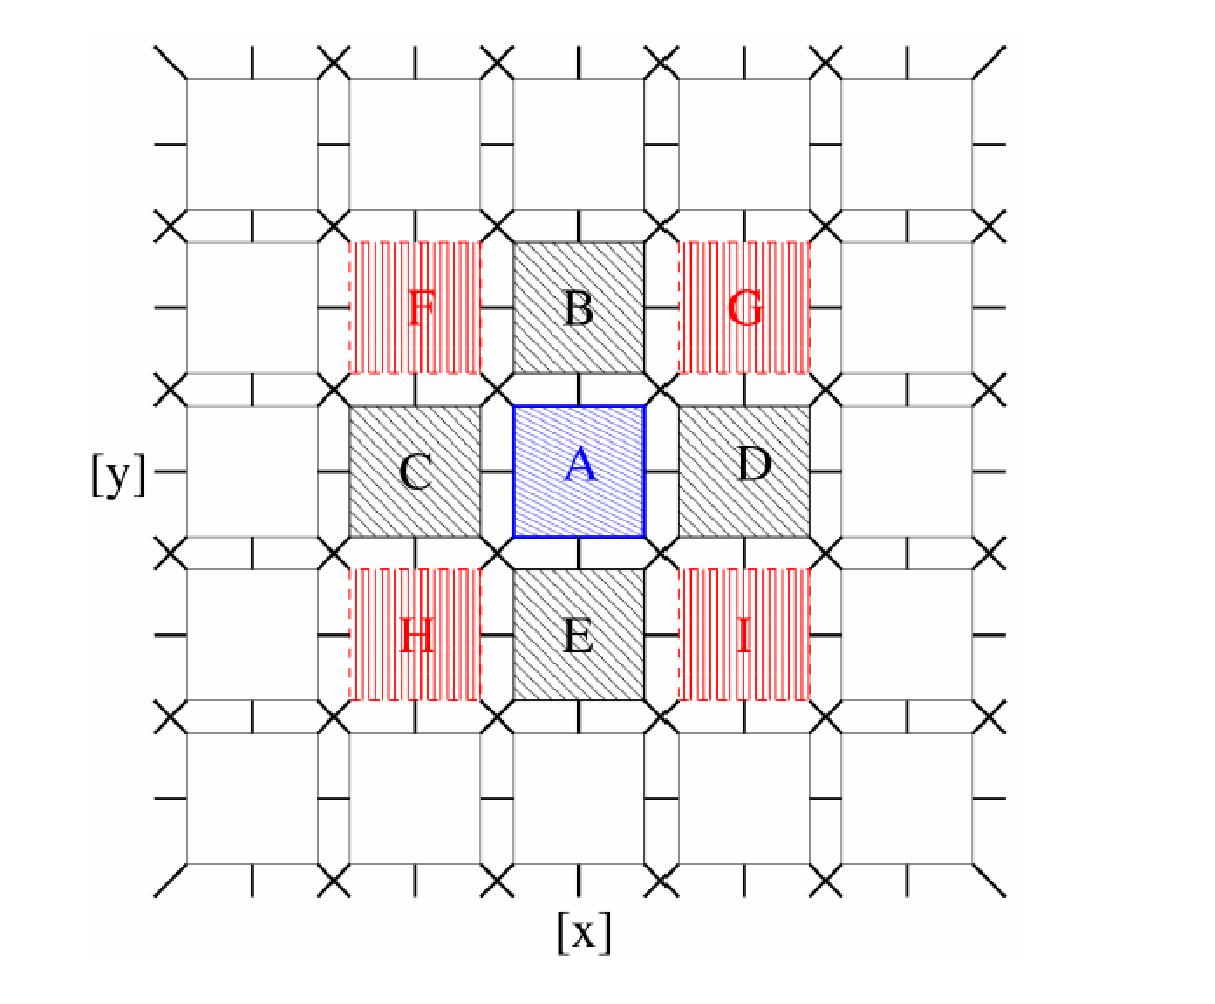
\includegraphics[width=0.5\textwidth]{pics/spatialprison}
  \label{prison}
  \caption{Spatial Prisoner's Dilemma.}
\end{figure}

\subsection*{Exercises}

\begin{enumerate}
\item Implement the spatial prisoner's dilemma with the following
  payoff-matrix

  \begin{tabular}{l|cc}
    & cooperate & defect\\\hline
    cooperate & 7  & 0  \\
  defect    & 10 & 0  \\
  \end{tabular}

  on an $N\times N$ grid and run it for $n$ iterations.
  
  Create two $N\times N\times n$ numpy-arrays $S$ and $P$ and save for
  each cell and each iteration, the strategy applied by the cell and
  the received payoff.
\item Plot the strategy as $N\times N$-image for each iteration in a
  loop using {\tt ion()} and {\tt imshow()} such that you can see how
  the system evolves in a movie.
\item Plot the number of cooperating players by iteration.
\item Plot histograms for the distributions of
  \begin{enumerate}
  \item number of consecutive cooperations
  \item total number of cooperations over time
  \end{enumerate}
\item Experiment with different strategies to choose
  defection/cooperation. 
\end{enumerate}

\end{document}
